\chapter{Toolchain}\label{lab:toolchain}

    Das folgenden Kapitel beschreibt das Zusammenspiel verschiedener Softwarschichten
    um eine \textit{Toolchain} abzubilden die in der Lage ist, für den Softcore passenden
    Compilate zu erstellen, Speicherpartitionen zu generieren sowie den Bootloader
    zu erstellen und zu linken.
    Dafür wurde im Rahmen dieses Projektes ein, in \textit{GO} geschriebenes, Programm
    entworfen welches folgende Punkte in einem Programm vereint.
    Die Benutzung des Programmes wird in Kapitel \ref{lab:compile-code} beschrieben.

    \section{Compiler}

        Der \textit{Compiler} wird benötigt um Programmcode
        in \textit{RISC-V} Maschinenbefehle zu übersetzen.
        Zusätzlich formt dieser die Maschineninstruktionen in ein \textit{ELF}-Dateiformat
        (Siehe \ref{lab:elf}).\\
        Dazu wird die offene und freie
        \textit{GCC (GNU Compiler Collection)} verwendet.
        Das \textit{RISC-V} Team hat hierfür schon vorarbeitet geleistet und bietet
        den kompletten Toolchain Quellcode an.
        Dies ermöglicht das Bauen des \textit{Cross-Compilers} sowie von hilfreichen
        Zusatzprogrammen \cite{riscv-toolchain}.
        
    \subsection{Executable and Linkable Format (ELF)}\label{lab:elf}
        Das \textit{Executable and Linkable Format (ELF)} definiert ein
        standard Binärformat für ausführbare Programme, Bibliotheken sowie von
        Speicherauszügen. Jede \textit{ELF} besteht aus Kopfinformationen (Header)
        gefolgt von Daten. Die Kopfinformationen beinhalten Informationen 
        über die eigentlichen Daten. Dazu zählen bspw. Wordbreite, Byte-Reihenfolge,
        Elf-Typ oder Maschinentyp.\\
        Zu den Daten gehören unter anderem \textit{Sections Headers}.
        Diese beinhalten dabei Informationen über mehrere Code-Sektionen
        und deren Zugriffsrechte. Die eigentlichen Daten liegen dabei unter \textit{Data}.
        Die vier wichtigsten Sektionen für ausführbare Programme sind dabei folgende.
        
        \begin{description}
            \item[.text] ausführbarer Programmcode (Instruktionen)
            \item[.data] Initialisierte Daten mit Schreib- sowie Lesezugriff
            \item[.rodata] Initialisierte Daten mit Lesezugriff (Konstanten)
            \item[.bss] Uninitialisierte Daten (mit nullen initialisiert)
        \end{description}
    
    \subsection{Linker}
        Der Linker ist, im Kontext dieser Arbeit, vorallem dafür zuständig
        die Speicheranordnung zu definieren. Dafür werden die \textit{Sections} (Siehe \ref{lab:elf})
        in eine Reihenfolge gebracht die für die Hardware passt.
        Listing \ref{lst:lds} zeigt das Linkerskript welches die Speicheranordnung definiert.
        \texttt{ENTRY(\_start)} definiert hierbei den Einstiegspunkt (Siehe \ref{lab:bootloader}).
        \texttt{MEMORY} beschreibt die Speichergröße, sodass der Compiler weiß wie
        viel Speicher ihm zu Verfügung steht. Aufgrund der gewählten \textit{modifizierten Havard-Architekur} (Siehe \ref{lab:havard})
        gibt es nur einen Speicherpool, sodass Instruktionen sowie Daten zusammen liegen.
        In \texttt{SECTIONS} wird die Reihenfolge der Instruktionen und der Daten innerhalb des Speicher
        definiert. Im ersten Bereich stehen die Instruktionen (\texttt{.text}) gefolgt von den Konstanten (\texttt{.rodata}).
        Als nächstes folgen die Variablen (\texttt{.data}) sowie die Null-initialisierten Variablen (\texttt{.bss}).
        
        \lstinputlisting[style=cstyle,caption={Linkerskript},label=lst:lds]{../../Firmware/linker.lds}

    \section{Bootloader}\label{lab:bootloader}

        Der Bootloader ist in Assembler geschrieben und ist dazu da den
        Softcore zu initialisieren, sodass dieser bereit ist, Programmcode auszuführen.
        Dabei wird hauptsächlich die Stackadresse gesetzt und die \textit{Main}
        Funktion des C-Codes aufgerufen  (Listing \ref{lst:crt0s}).
        Hierbei ist zu beachten, dass der Stack von hinten nach vorne wächst.
        Aus diesem Grund wird als Stackadresse das letzte adressierbare Byte (0xFFFF) benutzt.
        \lstinputlisting[style=cstyle,caption={Bootloader crt0.s},label=lst:crt0s]{../../Firmware/crt0.s}

    \section{MIF Generierung}

        Die zugrunde liegende Speicherarchitektur (Siehe \ref{lab:memory})
        und deren Initialisierung (Siehe \ref{lab:elf}) benötigt vier \textit{MIF's}
        die durch die Toolchain generiert werden. Hierfür wird,
        vergleichbar mit dem Round-Robin-Verfahren, jedes Byte eines Words
        in einer unterschiedliche MIF geschrieben.

        \begin{figure}[H]
            \centering
            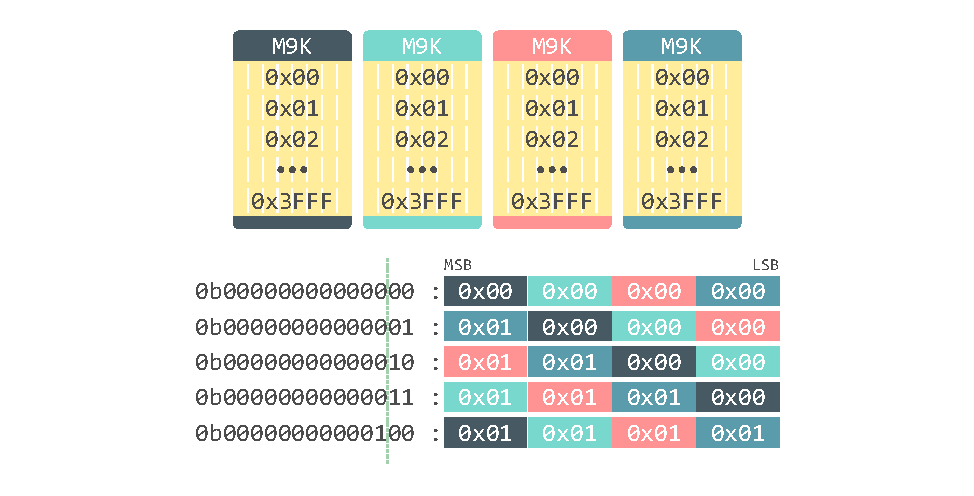
\includegraphics[scale=1]{img/memorypartition.pdf}
            \caption{Speicherpartitionen}
            \label{fig:memorypartition}
        \end{figure}
        
        
        
       